\newpage
\section{The SegmentAnalyser class} \label{sec:sa}

The class SegmentAnalyser offers post-processing methods per root segment. The advantage is that we can do distributions or densities, and that we can analyse the segments within any geometry. 

We start with a small example plotting the root surface densities of a root system versus root depth.

\subsection{Root surface densities}

\lstinputlisting[language=Python, caption=Example 3a]{../../examples/python/example3a_density.py}

\begin{figure}
\centering
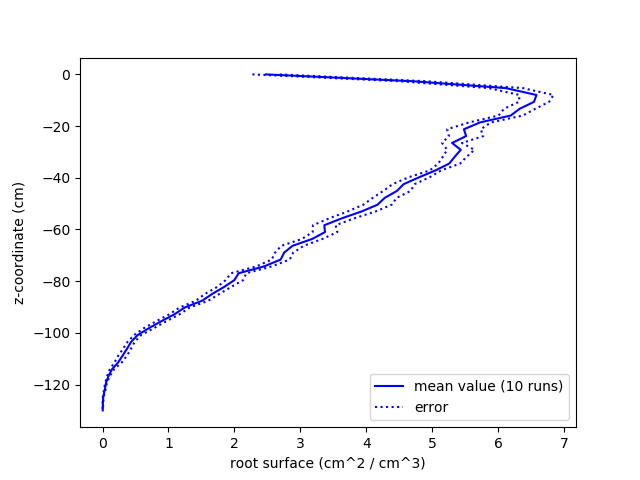
\includegraphics[width=0.7\textwidth]{example_3c.png}
\caption{Root surface densitiy versus depth(Example 3a)} \label{fig:surface_density}
\end{figure}


\begin{itemize}

\item[8-12] Pick a root system.
\item[14-16] Depth describes the y-axis of the graph, layers the number of vertical soil layers, where the root surface is accumulated, and runs is the number of simulation runs. 
\item[18-23] Performs the simulations. L23 creates a distribution of a parameter (name) over a vertical range (bot, top). The data are accumulated in each layer, segments are either cut (exact = True) or accumulated by their mid point (exact = False). 
\item[25] In order to calculate a root surface density from the summed up surface, we need to define a soil volume. The vertical height is the layer length, length and width (here 10 cm), can be determined by planting width, or by a confining geometry. 
\item[26-28] Calculates the densities mean and the standard error. 
\item[30-39] Prepares the plot (see Figure \ref{fig:surface_density}).

\end{itemize}



\subsection{Analysis per segment within a geometry}

The following script demonstrates some of the post processing possibilities by setting up a virtual soil core experiment (see Figure \ref{fig:soilcoreGeom}), where we analyse the content of two soil cores located at different positions.

\lstinputlisting[language=Python, caption=Example 3b]{../../examples/python/example3b_sdfanalysis.py}

\begin{itemize}

\item[11-15] Performs the simulation.

\item[17-22] We define two soil cores, one in the center of the root and one 10 cm translated. In L22 we pick which one we use for the further analysis. Figure \ref{fig:soilcoreGeom} shows the resulting geometry, with a soil core radius of 10 cm.

\item[24-28] Prepares three sub-figures. 

\item[31-41] Creates a root length distribution versus depth at different ages. L33 creates the SegmentAnalyser object, and L34 crops it to a fixed domain or maps it into a periodic domain. In L38 the filter function keeps only the segments, where the parameter (first argument) is in the range between second and third argument. L39 creates the distribution. 

\item[44-54] We repeat the procedure, but we crop to the soil core selected in L22. 

\item[57-89] In the third sub plot we make densities of specific root types like basal roots, first order roots, and second order roots. In L58 we crop the segments to the soil core geometry. In L63 we filter for the selected sub type, and in L64 we create the density distribution.

\item[71-73] Show and save resulting Figure \ref{fig:central} and \ref{fig:shifted} for the two soil cores (chosen in L22).

\end{itemize}

\begin{figure}
\centering
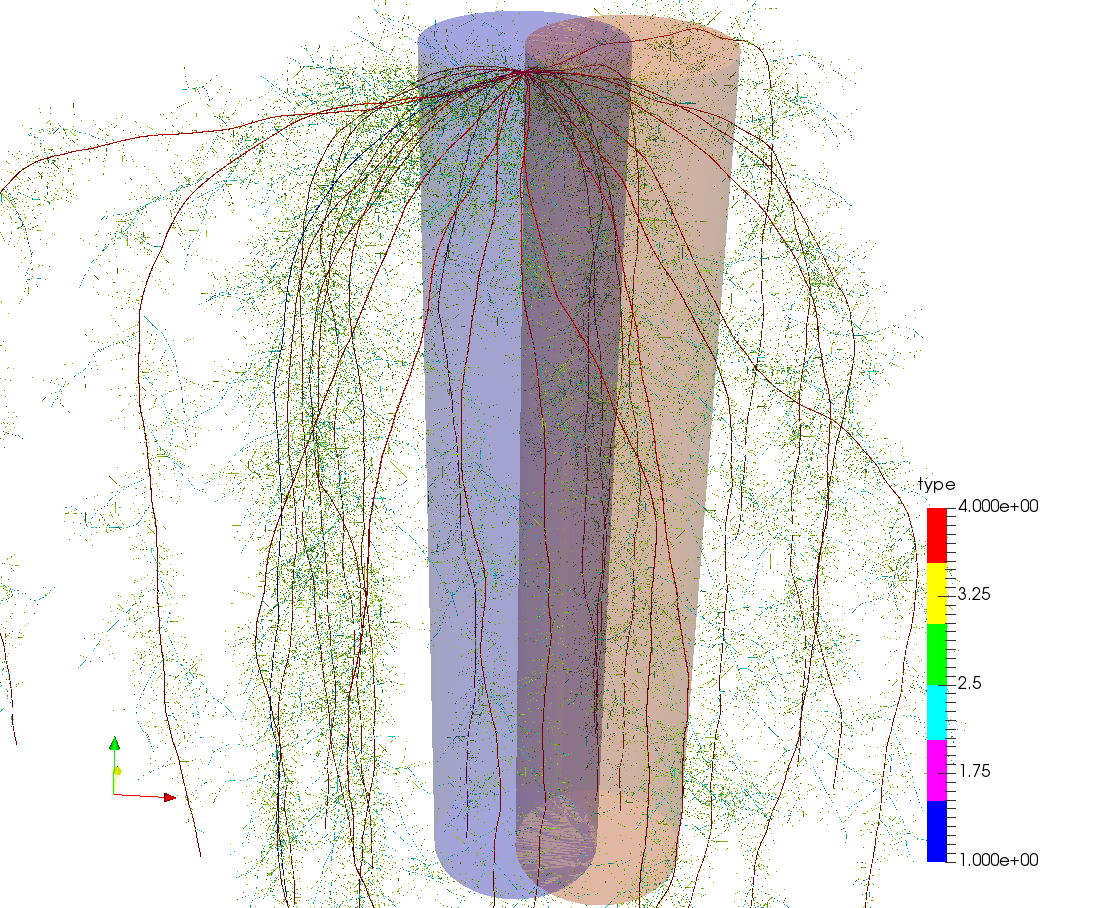
\includegraphics[width=0.7\textwidth]{example_3d.png} % 
\caption{Virtual soil cores experiment (Example 3b): Central core (blue), shifted core (red)} \label{fig:soilcoreGeom}
\end{figure} 


The example shows differences between the central core and shifted core (see Figure \ref{fig:central} and \ref{fig:shifted}) because the central core captures all roots emerging from the seed. The basic idea is that such analysis can help to increase the understanding of variations in experimental observations.

\begin{figure}
\centering
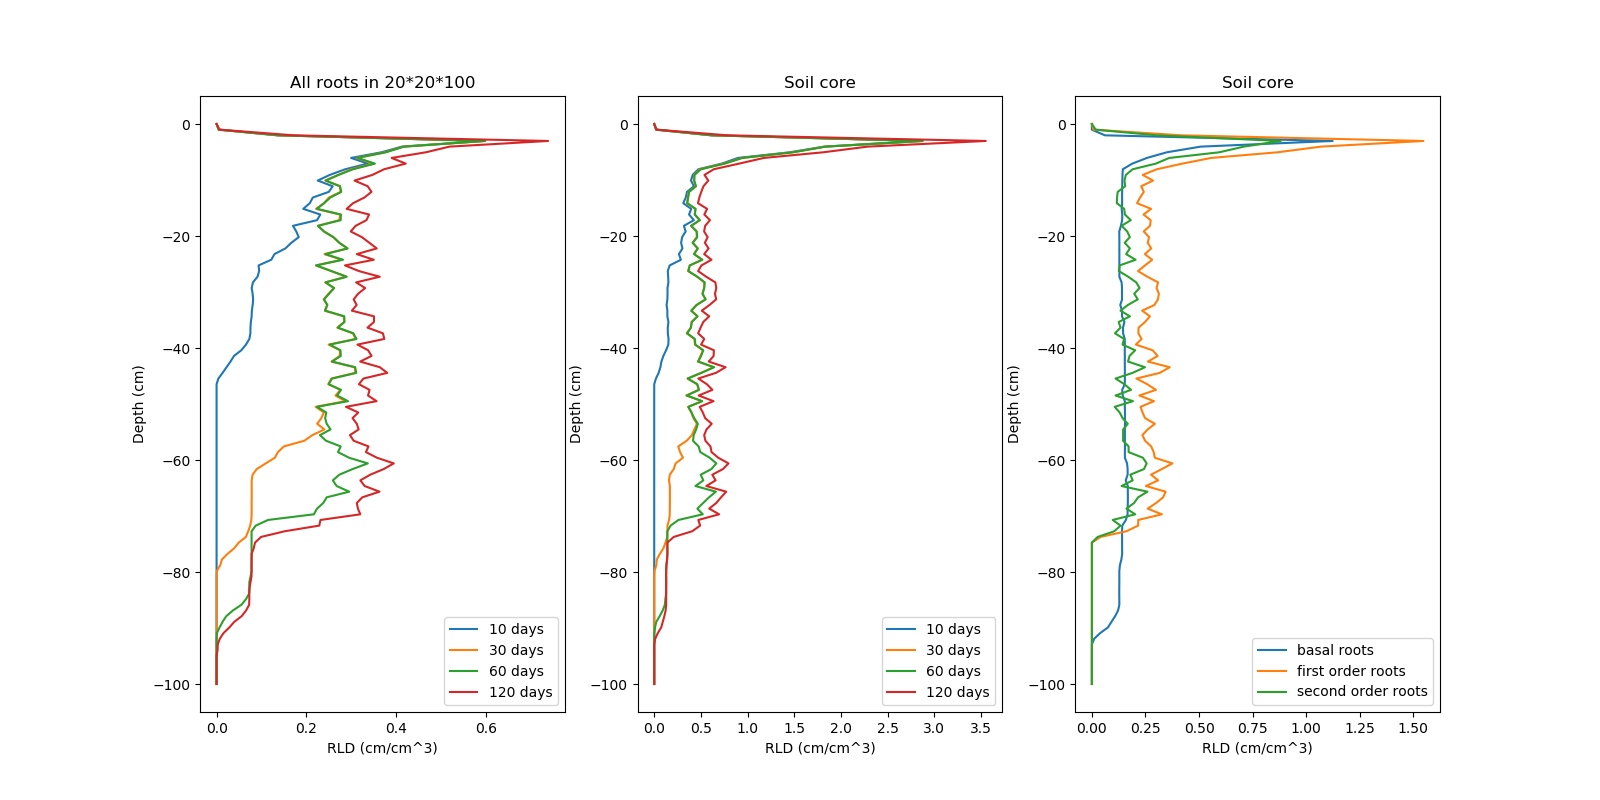
\includegraphics[width=0.9\textwidth]{example3b.png} 
\caption{Central core (Example 3b)} \label{fig:central}
\end{figure}

\begin{figure}
\centering
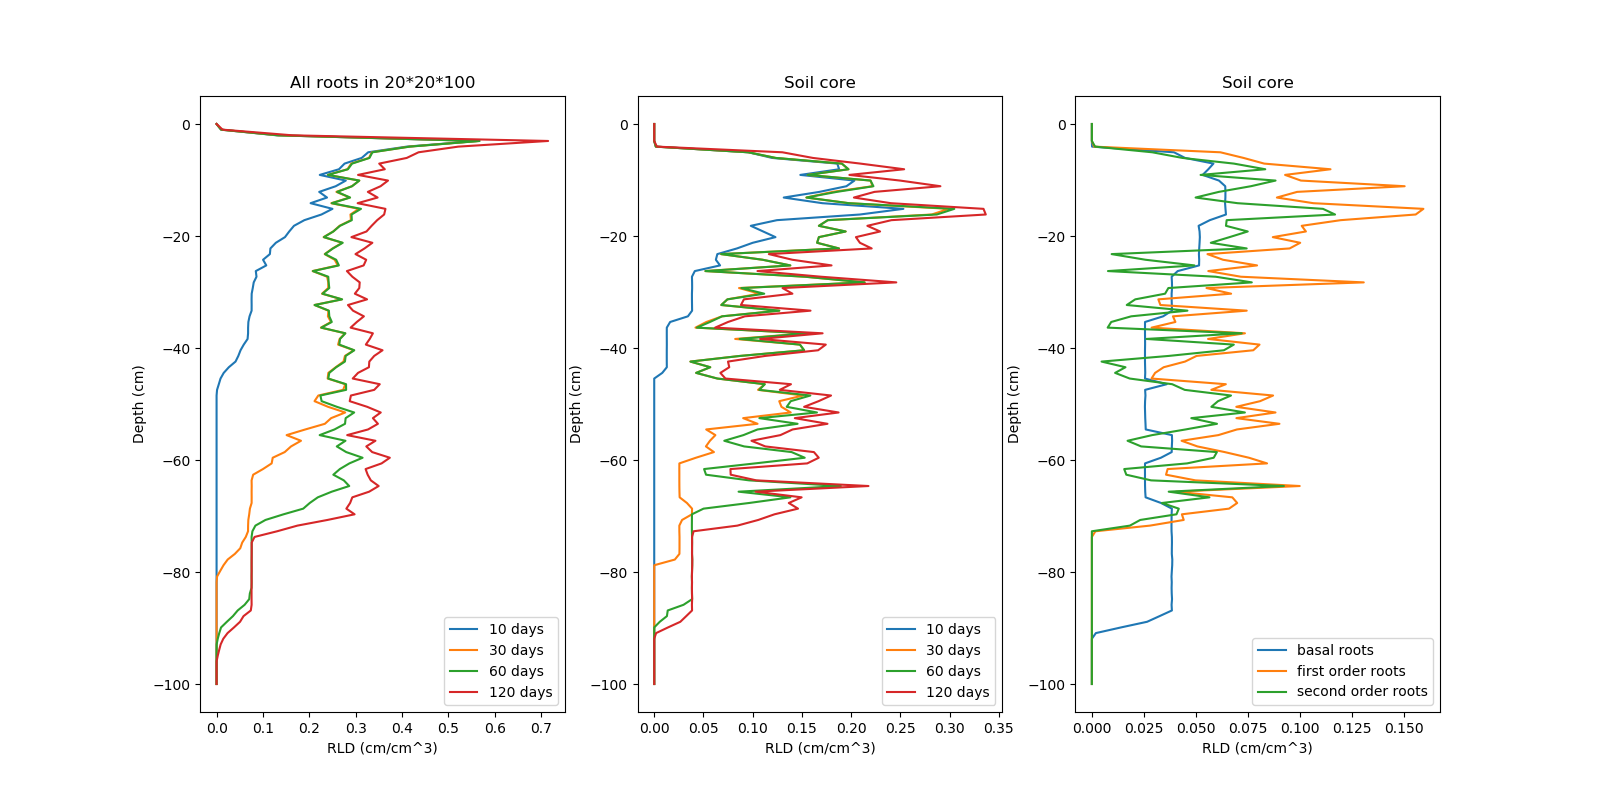
\includegraphics[width=0.9\textwidth]{example3b2.png} 
\caption{Shifted core (Example 3b)} \label{fig:shifted}
\end{figure}


\subsection{SegmentAnalyser for DGF or VTP export}

If we want to export our root system as dune grid file (dgf) we need to introduce an artificial shoot. By default the tap root and basal root starts at the seed node (i.e. multiple segments start at the same node), and its difficult to define a boundary condition for such a situation (e.g. in DuMux). Furthermore, if there are shoot borne roots, they emerge out of nothing above the seed node. Therefore, we introduce artificial segments eventually connecting shoot borne roots (if there are any) and connecting the seed node that is normally located at (0,0,-3) to the origin at (0,0,0). The following code snippet shows how to export a root system as dgf file:

\lstinputlisting[language=Python, caption=Example 3c]{../../examples/python/example3c_write.py}

\begin{itemize}
 \item[6-11] Defines a root sytem
 \item[13] Create the analyser object
 \item[15-18] Get the artificial shoot segments from the root system (L15) and manually add them to the SegmentAnalyser (L18), first argument is the segment $s$, second is creation time, third is radius, and fourth arguments states that the segment is inserted at the top of the list (True), while (False) would append it to segment list.
 \item[19] Write the VTP file. For VTP files its possible to add a list of parameters that will be exported. 
 \item[20] Write the DGF file. The parameters are fixed (see documentation of SegmentAnalyser::writeDGF)
\end{itemize}

It is also possible to make use of the SegmentAnalyser class without any other CPlantBox classes (e.g. for writing vtp from measurements). The following example shows how to construct the class with arbitrary nodes and segments (e.g. from measurements). 

\lstinputlisting[language=Python, caption=Example 3d]{../../examples/python/example3d_measurements.py}

\begin{itemize}
 \item[6-9] Define some segments with data
 \item[12,13] We convert the Python list to lists of C++ types
 \item[16] We create the SegmentAnalyser object without an underlying Organism
 \item[18,19] Use the Analyser object, by printing information, or writing a vtp. 
\end{itemize}

Next, we describe how to make an animation from a CPlantBox simulation.


\subsection{How to make an animation} \label{ssec:animation}

In order to create an animation in Paraview we have to consider some details. The main idea is to export the result file as segments using the class SegmentAnalyser. A specific frame is then obtained by thresholding within Paraview using the segments creation times. In this way we have to only export one vtp file. 

We modify example1b.py to demonstrate how to create an animation.

\lstinputlisting[language=Python, caption=Example 4c (modified from Example 1b)]{../../examples/python/example3e_animation.py} 

\begin{itemize}

\item[11,12] Its important to use a small resolution in order to obtain a smooth animation. L18 set the axial resolution to 0.1 cm. 

\item[19,29] Instead of saving the root system as polylines, we use the SegmentAnalyser to save the root system as segments.

\item[22,23] It is also possible to make the root system periodic in the visualization in $x$ and $y$ direction to mimic field conditions.

\item[26-28] We save the geometry as Python script for the visualization in ParaView.

\end{itemize}

After running the script we perform the following operations Paraview to create the animation:
\begin{enumerate}
 \item Open the .vtp file in ParaView (File$\rightarrow$Open...), and open tutorial/examples/python/results/example\_3e.vtp.
 \item Optionally, create a tube plot with the help of the script tutorial/pyscript/rsTubePlot.py (Tools$\rightarrow$Python Shell, press 'Run script').
 \item Run the script tutorial/pyscript/rsAnimate.py (Tools$\rightarrow$Python Shell, press 'Run script'). The script creates the threshold filter and the animation. 
 \item Optionally, visualize the domain boundaries by running the script tutorial/examples/python/results/example\_4e.py (Tools$\rightarrow$Python Shell, press 'Run script'). Run after the animation script (otherwise it does not work).  
 \item Use File$\rightarrow$Save Animation... to render and save the animation. Pick quality ($<$100 \%), and the frame rate in order to achieve an appropriate video length, e.g. 300 frames with 50 fps equals 6 seconds. The resulting files might be uncompressed and are very big. The file needs compression, for Linux e.g. ffmpeg -i in.avi -vcodec libx264 -b 4000k -an out.avi, produces high quality and tiny files, and it plays with VLC.
\end{enumerate}




